\documentclass[UTF8,a4paper,8pt]{ctexart} 

\usepackage{graphicx}%学习插入图
\usepackage{verbatim}%学习注释多行
\usepackage{booktabs}%表格
\usepackage{geometry}%图片
 \usepackage{amsmath} 
 \usepackage{amssymb}
   \CTEXsetup[format+={\flushleft}]{section}
%设置文章宽度
\geometry{textwidth=18cm}
%设置页面布局
\pagestyle{plain}
\author{郑华}
\title{PaintProject 需求说明}

 %正文排版开始
 \begin{document} 
 	\maketitle
   
   \section{项目概述}
      随着人们对生活水平的追求,人们使用手机的要求也随之提高,譬如说对操作的 简便 性,直观性,统一性等的进一步要求。所以说 这款画图软件将为人们解放一只手,为操作带来娱乐,直观,简单方便的 操作体验,同时不失去 基本操作的目标功能。

      而本系统目的是与手机2D涂鸦软件形成关联,使得用户在电脑上也可以对同一图元进行处理。
 
   \section{具体需求}	     
      \subsection{界面}
         首先用户界面得有以下特点:
       	\begin{enumerate}
       		\item 自己写窗口
       		\item 动态性
       		\item 美观
       		\item 与手机对应直观性
        \end{enumerate}
        
        	\begin{figure}[h] 	
        		\centering
        		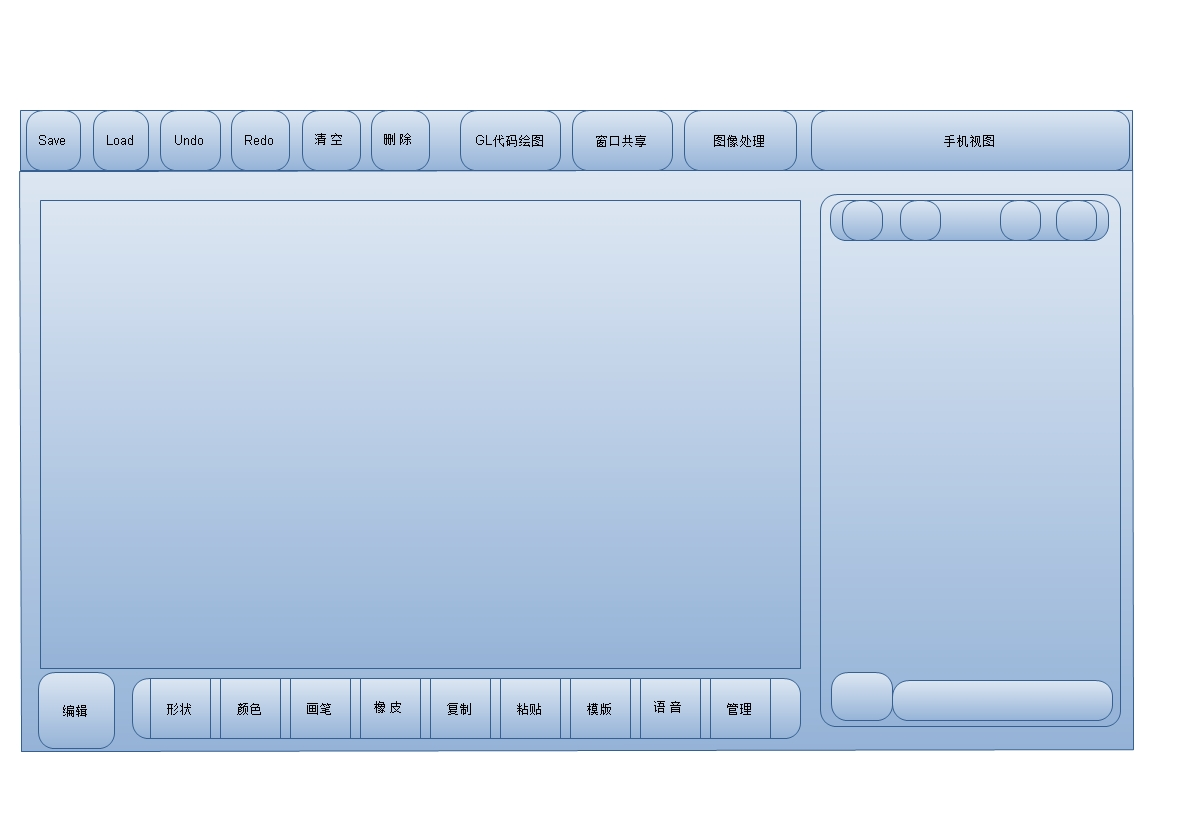
\includegraphics[width=8cm,clip]{MFC_PaintProjectIdea.jpg} 	
        		\caption{设计图}	
        		\label{fig:myphoto}
        	\end{figure} 
        	
      \subsection{功能}
       	\begin{enumerate}
        	\item 基本绘图
        	\item 对象的序列化
        	\item 网络传输
        	\item 画布的自由调节
        \end{enumerate}
      \subsection{具体细节}
      
      \paragraph{1- 绘图图形种类}:
      
       	\begin{enumerate}
       	  \item Line:直线
       	  \item BreakLine:折线
       	  \item Rect:矩形
       	  \item Oval:椭圆
       	  \item Circle:正规圆
       	  \item Hands:自由曲线
       	 \end{enumerate}
       	      	
      \paragraph{2- 笔刷的样式}
      
      	\begin{enumerate}
           \item Original
           \item SelfDefined
           \item Pen-
      	\end{enumerate}
      	
      \paragraph{3- 图元的复制粘贴}
        	\begin{enumerate}
        		\item  Copy
        		\item  Paste
        	\end{enumerate}
      \paragraph{4- 加载保存}
        	\begin{enumerate}
        		\item  Save
        		\item  Load
        	\end{enumerate}
      \paragraph{5- 图像处理}
         	\begin{enumerate}
         		\item  BinaryCode
         		\item  TemplateRecognize
         	\end{enumerate}
      
   \section{用户特点}
   
   
   \section{接口设计}
\end{document} 